\chapter{Problématiques émergentes}

L'une des principales innovations à apporter dans les infrastructures
d'applications sensibles au contexte réside dans l'introduction d'une interface
présentant un niveau d'abstraction élevé. Cela permetterait de représenter la
connectivité des composants applicatifs avec les politiques de haut niveau qui
la régissent.  Cette couche doit rester simple d'utilisation pour les
développeurs d'applications, et le modèle améliorer simultanément
l'automatisation et la sécurité.

\section{Ontologie de contexte}

\section{Théorie de promesse}

Le modèle permettant la définition des politiques d'administration serait un
modèle orienté sur les ontologies et basé sur la théorie de la promesse.
Celle-ci s'appuie sur un contrôle évolutif des objets intelligents,
contrairement aux modèles impératifs plus traditionnels pensés comme des
systèmes de gestion descendants.  Dans ces derniers, le gestionnaire central
doit être informé des commandes de configuration des objets sous-jacents et de
l'état actuel de ces objets.

Au sein du contexte, le modèle fournit une série d'objets qui définissent
l'application. Les objets englobent les terminaux, les groupes de terminaux et
les politiques qui définissent leur relation.

L'infrastructure conçoit un modèle d'objet pour le déploiement d'applications,
ces dernières constituant le point central. Historiquement, les applications
étaient limitées par les capacités du réseau et par des configurations visant à
prévenir leur utilisation abusive. Des concepts tels que l'adressage, le VLAN et
la sécurité sont depuis toujours intimement liés, ce qui limite l'évolutivité et
la mobilité des applications. Alors que les applications sont redessinées pour
la mobilité et l'évolutivité web, cette approche traditionnelle empêche leur
déploiement rapide et homogène.

\subsection{Principes de fonctionnement}

\section{Algorithmes de consensus}

\subsection{Algorithme de Paxos}

\subsection{Algorithme de Raft}

Raft est un algorithme de consensus qui est conçu pour être facile à comprendre.
Il est équivalent à Paxos dans la tolérance aux pannes et en termes de
performance. La différence, c'est qu'il est décomposé en sous-problèmes
relativement indépendants, et il traite de manière rigoureuse toutes les pièces
majeures nécessaires pour obtenir un système cohérent.

Le consensus est un problème fondamental dans les systèmes distribués tolérants
aux pannes. Consensus implique de multiples serveurs acceptant des valeurs. Une
fois qu'ils atteignent une décision sur une valeur, cette décision est
définitive. Les algorithmes de consensus typiques  sont amenés à faire des
progrès lorque la majorité de leurs serveurs sont disponibles, par exemple, un
cluster de 5 serveurs peut continuer à fonctionner même si deux serveurs ne sont
plus disponibles. Si plusieurs serveurs échouent, ils cessent de faire des
progrès (mais ils ne retournerons jamais de valeurs érronées)

\section{Vue d'ensemble}

Comme on le voit \ref{archi}

\begin{figure}[ht!]
  \centering
  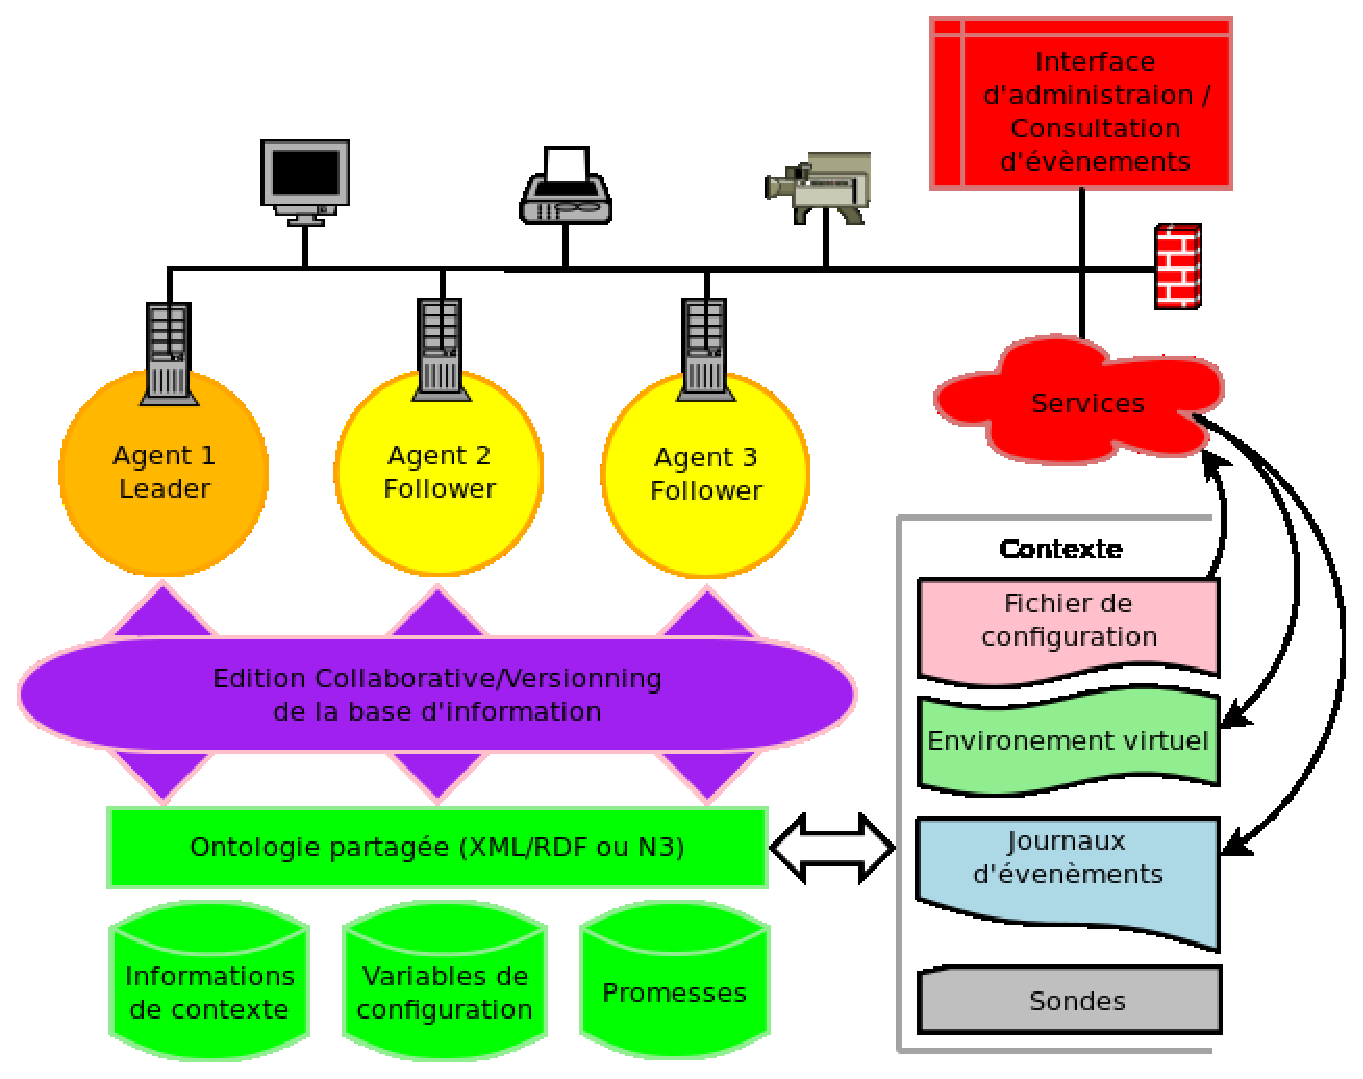
\includegraphics[width=90mm]{img/archi}
  \caption{Schéma d'implémentation du système multi-agents}
  \label{archi}
\end{figure}
